\chapter{Example: Quantum Speed Limit in Landau-Zener Model} \label{chap:LZexample}
To illustrate concepts from quantum optimal control theory, a state transfer within the Landau-Zener model is optimized using the GRAPE algorithm.\\
The Landau-Zener model is a two-level system with the general Hamiltonian
\begin{align}
	\hat{H}_{\mathrm{LZ}} = \begin{pmatrix}
    	 \Delta (t) & \Omega_R    \\
         \Omega_R & -\Delta (t) 		
    \end{pmatrix}  = \Omega_R \hat{\sigma}_x + \Delta (t) \hat{\sigma}_z \; , \label{eq:LZhamiltonian}
\end{align}
where $\Omega_R$ is the positive Rabi-frequency, $\Delta (t)$ is the detuning, and $\hat{\sigma}_i$ are the Pauli spin matrices. In such a system the detuning will be the control parameter, as it is easily to manipulate in an experimental setup. An advantage of the Landau-Zener system is that an analytical solution to the control problem exists for arbitrary initial and final states. Two level systems can be illustrated on the Bloch sphere, which depicts the population of the two levels along with the relative phases. Consider the transfer between the initial state
\begin{equation}
\lvert \psi_0 \rangle = \cos{\left(\frac{\theta_0}{2}\right)} \lvert 0 \rangle + e^{i\phi_0}\sin{\left(\frac{\theta_0}{2}\right)}\lvert 1 \rangle 
\end{equation}
and final state
\begin{equation}
\lvert \psi_T \rangle = \cos{\left(\frac{\theta_T}{2}\right)} \lvert 0 \rangle + e^{i\phi_T}\sin{\left(\frac{\theta_T}{2}\right)}\lvert 1 \rangle \; ,
\end{equation}
which are both expressed in terms of the angles of the Bloch sphere.
In CITE the quantum speed limit of such a state transfer was derived to be 
\begin{equation}
	T_{\mathrm{QSL}} = \lvert \frac{\theta_T - \theta_0}{2 \Omega_R} \rvert \; . 
\end{equation}
Consider the case of $\ket{\psi_0} = \ket{0}$ and $\ket{\psi_T} = \ket{1}$, whereby the quantum speed limit is $T_{\mathrm{QSL}} = \frac{\pi}{2 \Omega_R}$. 

\subsubsection{Optimal control using GRAPE} 
In this example $\Omega_R = 1$ for simplicity. Examining the Hamiltonian of eq. \eqref{eq:LZhamiltonian}, it is clear that the state transfer $\ket{0} \to \ket{1}$ can be achieved efficiently by letting $u(t) \equiv \Delta (t) = 0$ for the entire duration. To avoid this the control is subjected to the boundary conditions $u(0) = 0$ and $u(T) = 2 T$.\\
\begin{figure}[h!]
\centering % <-- add this
\begin{subfigure}[b]{0.48\textwidth}
	\caption{}  
  	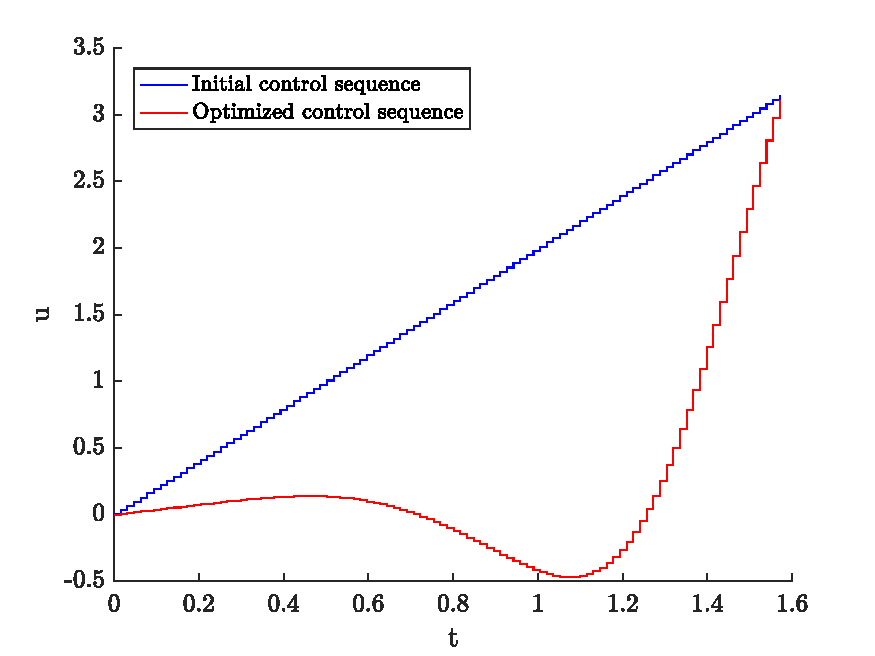
\includegraphics[width=\textwidth]{Figures/LZcontrol1.pdf}
\end{subfigure}
\hspace{3mm}
\begin{subfigure}[b]{0.48\textwidth}
	\caption{}    
  	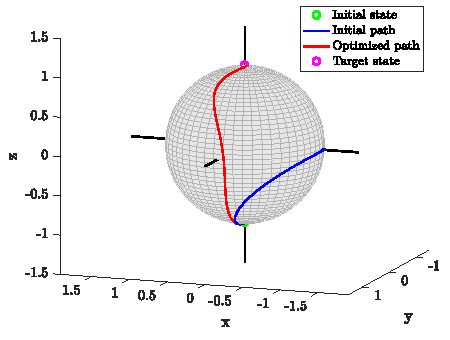
\includegraphics[width=\textwidth]{Figures/LZpath1.pdf}
\end{subfigure}

\caption{\textit{Optimal control of LZ-system using GRAPE for $T_1 = \pi / 2$. \textbf{(a)}: Initial and optimized control sequence. \textbf{(b)}: Path traced out on the Bloch sphere by the quantum state, as it is evolved according to the control.}}
\label{fig:LZopt1}
\end{figure}
Figure \ref{fig:LZopt1} displays the results of optimizing the state transfer using the GRAPE algorithm for duration $T_1 = \pi / 2$. The algorithm takes an initial linear seed, which clearly does not reach the target state. Clearly, the optimized control achieves perfect transfer. This is as expected, as the quantum speed limit for the transfer is $T_{\mathrm{QSL}} = T_1 = \pi / 2$, whereby a solution should exist for this duration. However, any duration shorter should not be sufficient to reach the target state.\\ 
\begin{figure}[h!]
\centering % <-- add this
\begin{subfigure}[b]{0.48\textwidth}
	\caption{}  
  	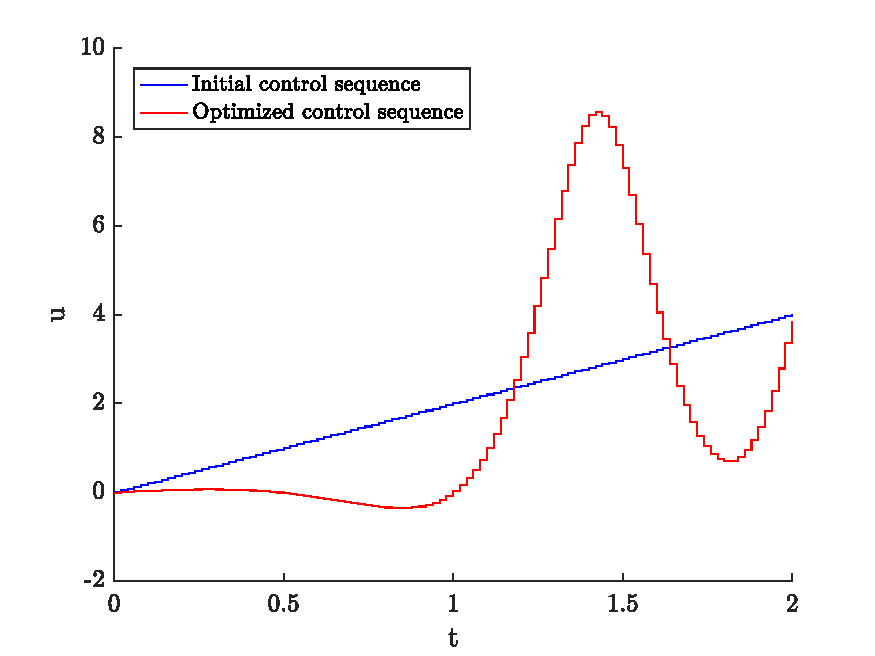
\includegraphics[width=\textwidth]{Figures/LZcontrol2.pdf}
\end{subfigure}
\hspace{3mm}
\begin{subfigure}[b]{0.48\textwidth}
	\caption{}    
  	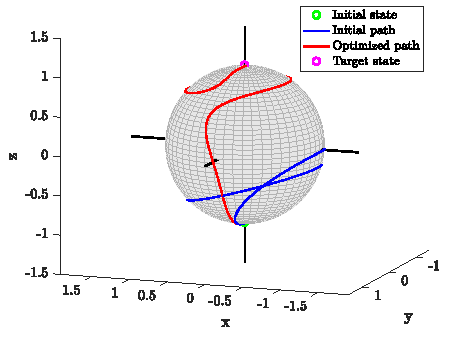
\includegraphics[width=\textwidth]{Figures/LZpath2.pdf}
\end{subfigure}

\caption{\textit{Optimal control of LZ-system using GRAPE for $T_2 = 2$. \textbf{(a)}: Initial and optimized control sequence. \textbf{(b)}: Path traced out on the Bloch sphere by the quantum state, as it is evolved according to the control.}}
\label{fig:LZopt2}
\end{figure}
Next, consider figure \ref{fig:LZopt2}, which shows the optimization results for duration $T_2 =  2$. As this duration is larger than the quantum speed limit, a solution exist for $T_2$. However, the path of the state on the Bloch sphere is much less direct than for the previous case. This is a consequence of how the optimal control is formulated, as one is searching for a control resulting in $\ket{\psi (T)} = \ket{\psi _{\mathrm{Target}}}$. Thus, the path of state has no impact on the cost.\\ For large duration solutions to the control problem generally become more abundant CITE. Figures \ref{fig:LZopt1} and \ref{fig:LZopt2} illustrate this point, as many different paths from $\ket{\psi _0} \to \ket{\psi _{\mathrm{Target}}}$ are possible for large durations, whereas only few possible solutions are available at durations close to the quantum speed limit.